%
% File acl2021.tex
%

\documentclass[11pt,a4paper]{article}
\usepackage[hyperref]{acl2021}
\usepackage{times}
\usepackage{latexsym}
\renewcommand{\UrlFont}{\ttfamily\small}
\usepackage{ctex}
\usepackage{multirow}
%\usepackage{parskip}
%\setlength{\parindent}{0cm}
\usepackage{graphicx}
\graphicspath{{figures/}}

% This is not strictly necessary, and may be commented out,
% but it will improve the layout of the manuscript,
% and will typically save some space.
\usepackage{microtype}

%\aclfinalcopy % Uncomment this line for the final submission
%\def\aclpaperid{***} %  Enter the acl Paper ID here

%\setlength\titlebox{5cm}
% You can expand the titlebox if you need extra space
% to show all the authors. Please do not make the titlebox
% smaller than 5cm (the original size); we will check this
% in the camera-ready version and ask you to change it back.
\usepackage{algorithm}  
\usepackage{algorithmicx}  
\usepackage{algpseudocode}  
\usepackage{amsmath}  

\newcommand\BibTeX{B\textsc{ib}\TeX}

\title{自然语言处理\quad 实验1\quad 汉语分词系统}


\begin{document}
	\maketitle
	\begin{abstract}
		本次实验目的是对汉语自动分词技术有一个全面的了解,包括从词典的建立、分词算法的实现、性能评价和优化等环节。本次实验所要用到的知识如下:基本编程能力(文件处理、数据统计等)、相关的查找算法及数据结构实现能力(如二分查找、Trie树、Hash表等等)、语料库相关知识、正反向最大匹配分词算法、N元语言模型相关知识以及分词性能评价常用指标(如准确率、召回率、F值等)。
	\end{abstract}
	
	\section{介绍}
	\label{Sec:Introduction}
	中文分词指的是将一个汉字序列切分成一个一个单独的词。分词就是将连续的字序列按照一定的规范重新组合成词序列的过程。我们知道,在英文的行文中,单词之间是以空格作为自然分界符的,而中文只是句段能通过明显的分界符来简单划界,而词是没有一个形式上的分界符的。虽然英文也同样存在短语的划分问题,不过在词这一层上,中文比之英文要复杂得多、困难得多。
	
	由于英文的语言使用习惯,通过空格我们很容易拆分出单词;而中文字词接线模糊往往不容易区别哪些是“字”,哪些是“词”。这也是为什么我们想把中文的词语进行切分的原因。
	
	当前研究所面临的问题和困难主要体现在三个方面:分词的规范、歧义词的切分和未登录词识别。
	
	\paragraph{分词的规范}
	
	中文因其自身语言特性的局限,字(词)的界限往往很模糊,关于字(词)的抽象定义和词边界的划定尚没有一个公认的、权威的标准。曾经有专家对母语是汉语者调查结果显示,对汉语文本中“词”的认同率仅有百分之七十左右。正是由于这种不同的主观分词差异,给汉语分词造成了极大的困难。尽管在1992年国家颁布了《信息处理用现代词汉语分词规范》,但是这种规范很容易受主观因素影响,在处理现实问题时也不免相形见绌。
	
	\paragraph{歧义词切分}
	
	中文中的歧义词是很普遍的,歧义词即同一个词有多种切分方式,该如何去处理这种问题。普遍认为中文歧义词有三种类型:
	\begin{enumerate}
		\item 交集型切分歧义,汉语词如AJB类型,满足AJ和JB分别成词。如“大学生”一种切分方式“大学/生”,另一种切分方式“大/学生”。你很难去判定那种切分正确,即使是人工切分也只能依据上下文,类似的有“结合成”、“美国会”等等。
		
		\item 组合型切分歧义,汉语词如AB,满足A,B,AB分别成词。如“郭靖有武功高超的才能”中的“才能”,一种切分“郭靖/有/武功/高超/的/才能”,另一种切分“中国/什么/时候/才/能/达到/发达/国家/水平”显示是不同的切分方式。
		
		\item 混合型切分歧义,汉语词包含如上两种共存情况。如“郭靖说这把剑太重了”,其中“太重了”是交集型字段,“太重”是组合型字段。
	\end{enumerate}
	
	
	\paragraph{未登录词识别}
	
	未登录词又称新词。这类词通常指两个方面,其一是词库中没有收录的词,其二是训练语料没有出现过的词。未登录词主要体现在以下几种:
	
	\begin{enumerate}
		\item 新出现的网络用词:如“屌丝”、“蓝牙”、“蓝瘦香菇”、“房姐”、“奥特”、“累觉不爱”等。
		
		\item 研究领域名称:特定领域和新出现领域的专有名词。如“苏丹红”、“禽流感”、“埃博拉”、“三聚氰胺”等。
		
		\item 其他专有名词:诸如城市名、公司企业、职称名、电影、书籍、专业术语、缩写词等。如“成都”、“阿里巴巴”、“毛主席”、“三少爷的剑”、“NLP”、“川大”等。
	\end{enumerate}
	
	综述所述,处理汉语词边界、歧义词切分和未登录词切分问题比较复杂,其中未登录词的影响大大超过了歧义词的影响,所以如何处理未登录词是关键问题。
	
	本文将在课堂学习汉语自动分词原理和方法基础上,实现汉语分词的若干关键技术,包括词典的构建、正反向最大匹配分词、效果分析、基于统计语言模型的分词系统等环节。
	
	\section{相关工作}
	早在80年代就有中文分词的研究工作,曾有人提出“正向最大匹配法”、“逆向最大匹配法”、“双向扫描匹配法”、“逐词遍历法”等方法,共计多达16种之多。由于这些分词方法多是基于规则和词表的方法,随着统计方法的发展,不少学者提出很多关于统计模型的中文分词方法。关于规则的中文自动方法主要包括基于字符串匹配的分词方法、基于理解的分词方法和基于统计的分词方法。
	
	\paragraph{基于字符串匹配的分词方法}
	基本思想是基于词典匹配,将待分词的中文文本根据一定规则切分和调整,然后跟词典中的词语进行匹配,匹配成功则按照词典的词分词,匹配失败通过调整或者重新选择,如此反复循环即可。代表方法有基于正向最大匹配和基于逆向最大匹配及双向匹配法~\citep{edmonds1965maximum}。
	
	\paragraph{基于理解的分词方法}
	基本思想是通过专家系统或者机器学习神经网络方法模拟人的理解能力。前者是通过专家对分词规则的逻辑推理并总结形成特征规则,不断迭代完善规则,其受到资源消耗大和算法复杂度高的制约。后者通过机器模拟人类理解的方式,虽可以取得不错的效果,但是依旧受训练时间长和过拟合等因素困扰。
	
	\paragraph{基于统计的分词方法}
	统计的中文分词方法包括:
	
	\begin{enumerate}
		\item 
		基于隐马尔可夫模型的中文分词方法。基本思想是通过文本作为观测序列去确定隐藏序列的过程。该方法采用Viterbi算法对新词识别效果不错,但具有生成式模型的缺点,需要计算联合概率,因此随着文本增大存在计算量大问题。
		\item 基于最大熵模型的中文分词方法。基本思想是学习概率模型时,在可能的概率分布模型中,认为熵最大的进行切分。该法可以避免生成模型的不足,但是存在偏移量问题。
		\item 基于条件随机场模型的中文分词方法。基本思想主要来源最大熵马尔可夫模型,主要关注的字跟上下文标记位置有关,进而通过解码找到词边界。因此需要大量训练语料,而训练和解码又非常耗时。
	\end{enumerate}
	
	综上所述,关于词典和规则的方法其分词速度较快,但是在不同领域取得效果差异很大,还存在构造费时费力、算法复杂度高、移植性差等缺点。基于统计的中文分词,虽然其相较于规则的方法取得不错的效果,但也依然存在模型训练时间长、分词速度慢等问题。针对这些问题,本文提出基于隐马尔可夫统计模型和自定义词典结合的方法,其在分词速度、歧义分析、新词发现和准确率方面都取得不错效果。
	
	\section{最大匹配分词——石翔宇}
	
	我们将在本节分别介绍词典的构建、正反向最大匹配分词、分词结果的评价的具体细节。
	
	\subsection{词典的构建}
	词典是分词任务的基础,没有词典的分词任务就如无源之水。我们将训练集中的词性和所有辅助标注的符号去除掉,得到单个词。
	
	需要注意的是,我们并不是将训练集的所有词都加到词典中。首先,训练集中每行开头的信息不加入词典。其次,训练集中重复的词不加入词典。这样不仅可以减少词典的噪声,同时也提高了词典的时空性能。
	
	不同的分词方法对词典的要求不同。有的方法只要求词典中包含词即可,我们将这样的词典称为零元词典。而有的方法需要词典统计出各个词的出现频率,称之为一元词典。有的方法甚至需要统计出各个词及其前一个词共同出现时的频率,被称之为二元词典。
	
	形式化地,我们定义词典的容量为$N$,单个词为$w_i,\ i=1, 2, \dots, N$,词$w_i$的出现频率为$P(w_i)$,词$w_i$及其前一个词$w_{i-1}$共同出现的频率为$P(w_i|w_{i-1})$。则零元词典的每个条目为
	\begin{equation}
		w_i,\quad i=1, 2, \dots, N
	\end{equation}
	一元词典的每个条目为
	\begin{equation}
		w_i\ P(w_i),\quad i=1, 2, \dots, N
	\end{equation}
	二元词典的每个条目为
	\begin{equation}
		w_i\ P(w_i|w_{i-1}),\quad i=1, 2, \dots, N
	\end{equation}
	
	\subsection{正反向最大匹配分词}
	最大匹配分词~\citep{edmonds1965maximum}基于一种非常朴素的思想,对于每个分割出来的词组,我们总是希望这个词组的长度是最大的。其主要原理都是首先切分出单字串,然后和词典进行比对,如果当前切分是一个词那么就记录下来,否则通过增加或者减少一个单字,继续比较,一直还剩下一个单字则终止,如果该单字串无法切分,则作为未登录处理。
	
	顾名思义,正向最大匹配分词就是从待分单句的前面开始,按照词典中的词进行切分,直到切分完成。而反向最大匹配分词则是从待分序列的末尾开始,按照词典中的词进行切分,直到切分完成。
	
	该算法的朴素时间复杂度为$O(L^2)$,但经过优化可以降低到$O(kL)$,其中$k$为词典中词的最大长度。
	
	\subsection{正反向最大匹配分词中词典的结构}
	线性存储的词典在查找时将会带来巨大的时间开销,有时这样的时间开销是我们无法接受的。在本节中将使用Trie树、平衡二叉树和哈希表来改进存储词典的数据结构以获取可接受的时间性能。
	
	\subsubsection{Trie树}
	在计算机科学中Trie树~\citep{thue1912uber},又称前缀树或字典树,是一种有序树,用于保存关联数组,其中的键通常是字符串。与二叉查找树不同,键不是直接保存在节点中,而是由节点在树中的位置决定。一个节点的所有子孙都有相同的前缀,也就是这个节点对应的字符串,而根节点对应空字符串。一般情况下,不是所有的节点都有对应的值,只有叶子节点和部分内部节点所对应的键才有相关的值。
	
	Trie树有如下的基本性质:
	\begin{enumerate}
		\item 根节点不包含字符,除根节点意外每个节点只包含一个字符。
		\item 从根节点到某一个节点,路径上经过的字符连接起来,为该节点对应的字符串。
		\item 每个节点的所有子节点包含的字符串不相同。
	\end{enumerate}
	
	Trie树可以最大限度地减少无谓的字符串比较,故可以用于词频统计和大量字符串排序。
	
	最大匹配分词中,我们只需将当前待处理字符串在trie树中比较,直到无法匹配为止,停下来的位置就是词典中的当前字符串的最大匹配子串。
	
	\subsubsection{平衡二叉树}
	平衡二叉树一般是一个有序树,它具有二叉树的所有性质,其遍历操作和二叉树的遍历操作相同。但是由于其对二叉树施加了额外限制,因而其添加、删除操作都必须保证平衡二叉树的因子被保持。
	
	平衡二叉树中引入了一个概念:平衡二叉树节点的平衡因子。它指的是该节点的两个子树,即左子树和右子树的高度差,即用左子树的高度减去右子树的高度,如果该节点的某个子树不存在,则该子树的高度为$0$,如果高度差的绝对值超过$1$就要根据情况进行调整。
	
	最大匹配分词中,我们可以用平衡二叉树来对Trie树的当前节点的子节点进行查找,可以将时间复杂度从$O(n)$降到$O(\log n)$。
	
	\subsubsection{哈希表}
	
	哈希表又称散列表,是除顺序表存储结构、链接表存储结构和索引表存储结构之外的又一种存储线性表的存储结构。
	
	哈希表存储的基本思路是:设要存储的对象个数为$n$,设置一个长度为$m(m\geq n)$的连续内存单元。以线性表中每个对象的关键字$k_i(0\leq i\leq n-1)$为自变量,通过一个称为哈希函数的函数$h(k_i)$,把$k_i$映射为内存单元的地址$h(k_i)$,并把该对象存储在这个内存单元中。
	
	最大匹配分词中,我们也可以用哈希表来对Trie树的当前节点的子节点进行查找,若能够选择合适的哈希函数,可以将时间复杂度从$O(n)$降到$O(1)$。
	
	
	\subsection{分词效果评价指标}
	
	\subsubsection{划分训练集和测试集}
	对于模型的评估与选择,我们可以通过实验测试来对学习器的泛化误差进行评估并对模型进行选择,因此我们需要一个测试集来测试学习器对没有见过的新样本的判别能力,并且用学习器在该测试集上的测试误差作为泛化误差的近似。
	
	测试集应该尽可能与训练集互斥,也就是说测试集中的样本尽量不在训练集中出现,也就是尽量不在训练过程中被使用过。因此,我们将整篇文本按9:1的比例划分为训练集和的测试集。
	
	\subsubsection{评价指标}\label{sxy:mec}
	我们使用准确率(Precision)、召回率(Recall)和F值(F ) 作为分词效果的评价指标,各指标的计算公式如下:
	\begin{equation}
		\begin{aligned}
			\text { Precision } &=\frac{T P}{T P+F P} \\
			\text { Recall } &=\frac{T P}{T P+F N} \\
			\text { F } &= \frac{2 \times \text { Precision } \times \text { Recall }}{ \text { Precision }+\text { Recall }}
		\end{aligned}
	\end{equation}
	$TP$表示将正样本预测为正样本,即预测正确;$FP$表示将负样本预测为正样本,即预测错误;$FN$表示将正样本预测为负样本,即预测错误。
	
	
	
	\section{最大匹配分词——王雨桐}
	\subsection{词典的构建}
	\noindent
	\textbf{词典}是基于字符串匹配分词算法的匹配依据,分词程序需要将待分词的语句拆分成长短不一的字符串,在词典中对其进行匹配。然而,词典中的词并不是越多越好,因为字典规模的扩大意味着匹配算法时间和空间复杂度的上升。尽管完善的词典有助于提高分词的准确性等指标,但在另一方面又会引起运行性能的下降。因此,我们所构建的词典,应是在词和分词单位基础之上考虑分词的性能,进行折衷之后做出的工程选择。换句话讲,在构建词典时,应当基于某种策略,对语料库中的信息做出适当的取舍,从而获得一个有用的数据占比较多的词典。在这里我生成词典的策略如下:
	
	\paragraph{不加入数词。}供我们构建词典的语料库中参杂着许多对于分词任务用处不大的冗余信息。例如在人民日报1998年1月的语料库中,每行文字之前都有一串标识段落的刊登日期和位置的数字,这些数字数量庞大且具有唯一性,对我们的分词程序几乎没有参考意义(如图\ref{num_word})。而正文部分也存在着许多规律性较差的数词,所以在构建词典时应优先将这些数词排除。
	
	\begin{figure}[htbp]
		\centering
		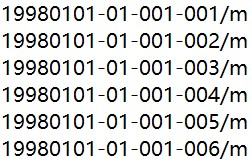
\includegraphics[width=5cm]{num_word.jpg}
		\caption{每行文本开头的数词}\label{num_word}
	\end{figure}
	
	\paragraph{不加入人名。}人名同数词一样,是一类重复出现几率较小、缺乏规律性的词,同样不会为我们使用词典进行分词的效果带来太大的提升。因此,在本节构建词典时暂不考虑加入人名,而是在性能冲刺环节中再对人名做额外的处理。
	
	\paragraph{保留地名。}地名在文档中出现的机会较多,且不同地名的数量远少于不同人名。值得注意的是,许多地名在文档中都是重复多次出现,如北京市、内蒙古自治区等等。在词典中保有一定量的地名信息,将有助于我们对文章中数量较多的地名进行分词。
	
	\paragraph{不引入频率。}这节构建的词典仅用于正向最大匹配分词(FMM)和反向最大匹配分词(BMM),因此在进行匹配时总是优先选择在词典中最长的词作为分词结果,而不是基于词出现的频率进行选择。因此,在本节构建词典时,暂不统计每个词在文中出现的频率。
	
	依照以上策略构建好词典后,便可以在其基础之上进行正反向最大匹配分词。\footnote{这里生成的词典仅用于3.5节之前,在3.5节中还会构建其他类型的辅助词典。}
	
	\subsection{正反向最大匹配分词实现}\label{chapter3.2}
	\noindent
	本节要求使用前面生成的词典实现正向最大匹配分词算法(FMM)和反向最大匹配分词算法~\citep{edmonds1965maximum}。下面给出FMM算法\ref{fmm_algo}和BMM算法\ref{bmm_algo}的伪代码:
	\floatname{algorithm}{算法}
	\renewcommand{\algorithmicrequire}{\textbf{输入:}}  
	\renewcommand{\algorithmicensure}{\textbf{输出:}}  
	\begin{algorithm}[h]
		\caption{正向最大匹配分词}\label{fmm_algo}
		\begin{algorithmic}[1] %每行显示行号  
			\Require $s$待分词的句子,$N$句子长度
			\Function{Fmm}{$s, N$}   
			\For{$i = 0 \to N-1$}
				\For{$j = N \to i+1$}
					\If {\Call{IsWord}{$s[i...j]$)}}
						\State \Call{Output}{$s[i...j]$}
						\State i $\gets$ j
					\EndIf
				\EndFor
				\State \Call{Output}{$s[i]$}
			\EndFor
			\EndFunction  
		\end{algorithmic}  
	\end{algorithm}

	\begin{algorithm}[t]
		\caption{反向最大匹配分词}\label{bmm_algo}
		\begin{algorithmic}[1] %每行显示行号  
			\Require $s$待分词的句子,$N$句子长度
			\Function{Bmm}{$s, N$}   
			\For{$i = N \to 1$}
				\For{$j = 0 \to i-1$}
					\If {\Call{IsWord}{$s[j...i]$)}}
						\State \Call{Output}{$s[j...i]$}
						\State i $\gets$ j
					\EndIf
				\EndFor
				\State \Call{Output}{$s[i-1]$}
			\EndFor
			\EndFunction  
		\end{algorithmic}  
	\end{algorithm}

	在以上两个算法中,{\bfseries\scshape IsWord()}函数的功能为在之前构建的词典中查找当前的句子切片。具体的数据结构实现方法为使用Python中的{\bfseries List}存储每个词典条目,查找字典时简单地调用{\bfseries in}方法在其上做线性搜索。
	
	除此之外,还需要对每行文字开头标识段落的刊登日期和位置的数字进行单独处理。由于构建的词典中不含有任何的数词,调用HMM和BMM算法时会将这串数字拆散成单独成词的一个个数字,这会造成准确率的急剧下降。因此,在对每行文本进行分词之前,先将行头的一整串数字取出,对剩余部分运行FMM和BMM算法,最后再将行头的数字作为一整个词插入到分词结果的前部,便可以解决这个问题。
	
	然而在实际运行基于以上思想实现的分词程序时,发现其时间性能方面的表现很差。由于生成的词典约含5万个条目,每次查找词典又是在词典空间中做线性搜索,会造成巨额的时间开销。使用该程序完成对2万余行文本的分词共耗时约4个半小时。显然这样的时间性能在实际运用中是不能被接收的,在对大量的文本信息进行分词时会陡然提升时间成本。因此,需要对储存词典的数据结构和查找算法进行改进,以提升程序的时间性能,这部分工作将在之后的第\ref{chapter3.4}节中完成。
	
	\subsection{正反向最大匹配分词效果分析}
	\noindent
	这部分内容请见\ref{wyt_analyzation}节。
	
	\subsection{基于机械匹配的分词系统的速度优化}\label{chapter3.4}
	\noindent
	通过前面的\ref{chapter3.2}节的实验结果可知,对词典进行线性存储,查找时使用线性查找的方法将会带来巨大的时间开销。因此,在本节中将改进存储词典的数据结构以及词典的查找算法,以获取可接受的时间性能。
	
	\paragraph{主体数据结构使用Trie树:}{\bfseries Trie树}~\citep{thue1912uber}是经常用于存储文本、编码等字符串信息的数据结构。树中每个结点存储一个字符,其所有子结点都以该结点作为其前缀字符,而树的根节点为空。也就是说,具有公共前缀的字符串同属一棵子树。例如,想要存储“我爱学习”、“我爱你中国”、“我是谁”、“你好”就可以使用以下的树结构进行存储:
	\begin{figure}[htbp]
		\centering
		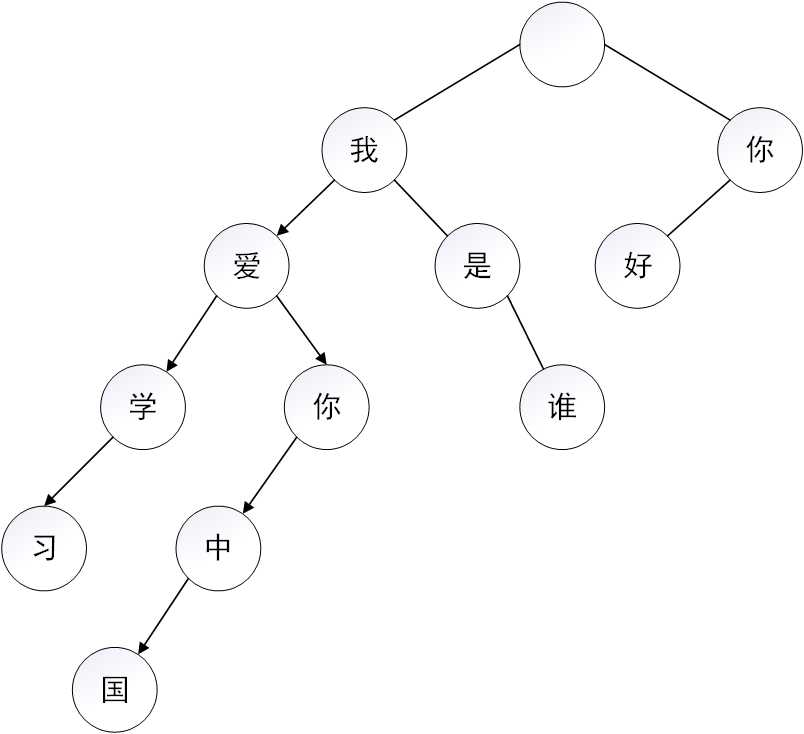
\includegraphics[width=7.5cm]{trie.png}
		\caption{Trie数结构举例}\label{trie}
	\end{figure}
	
	使用Trie树的好处在于,原来对词典进行线性搜索,假设词典中包含$n$个条目,则每在词典中查找一个词平均要进行$\frac{n}{2}$次操作,这一次数正比于词典中的条目数。这意味着,我们构建的词典越大,搜索所耗费的时间也就越多,时间性能也就越差。这不利于我们构建一个相对完善的词典。而如果使用Trie树存储词典,则树高就是词典中最长词的长度。也就是说,我们在Trie树中最多进行这一长度次数的匹配,就可得知当前的词是否存在于词典中。更可观的是,假设词典中的平均词长为3,则在Trie树中平均只需进行3次匹配。
	
	\paragraph{在每个结点使用哈希表存储子结点信息:}处理中文信息时,只使用传统的Trie树结构是不行的。对于英语来说,其字符集大小仅为26,因此Trie树中每个结点最多只有26个子结点(如果不考虑大小写及标点)。对于这一数量级,完全可以使用简单的列表等线性数据结构存储子结点的信息,并且很容易便可以将各字母一一映射到唯一的索引上去。然而,汉语中仅仅是常用字就有7000多个,这就意味着一个结点可能存在上千个子结点,尤其是根节点。我们既不能使用线性数据结构存储子结点的信息,因为这又会带来巨额的查找时间开销。又不能对汉字编码和索引做简单的一一映射,因为这会带来巨大的空间开销。所有的困难都指向了一个答案——使用{\bfseries 哈希表}。
	
	\begin{figure}[htbp]
		\centering
		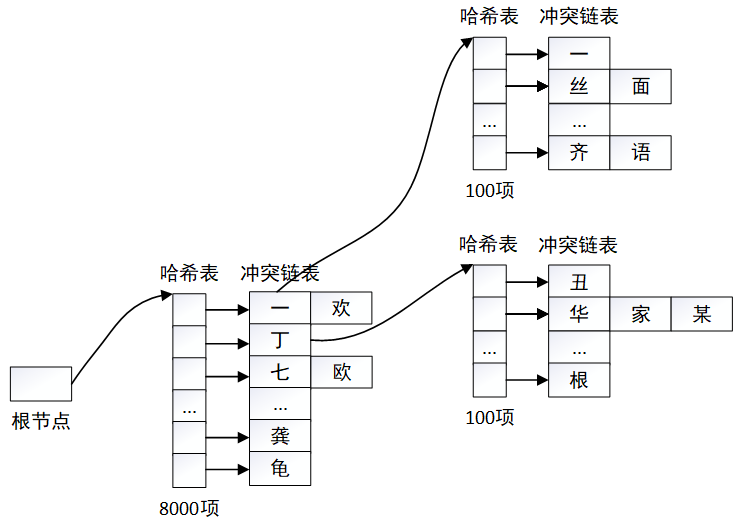
\includegraphics[width=7.5cm]{hash.png}
		\caption{哈希表数据结构}\label{hash}
	\end{figure}
	
	我在这里使用的冲突处理方法是开散列法,具体结构如图\ref{hash}所示。由于根节点的各子结点对应的是词典中所有词的第一个字,总数庞大,因此为其分配的哈希表大小为8000;其余各结点的子结点数量较少,为每个结点分配的哈希表大小为100。在进行索引映射时,采取的策略是将汉字的Unicode编码值对哈希表大小取余,即:
	\begin{equation}
		\mbox{索引值}=\mbox{Unicode编码值}\%\mbox{哈希表大小}
	\end{equation}
	\noindent 经测算,所有哈希表的冲突率都能控制在10\%以内。也就是说,$\frac{1}{10}$的几率需要在冲突链表上进行线性搜索,而实际上搜索空间一般不会超过3,这样的性能明显优于之前的线性搜索。
	
	经测量,对199801\_sent.txt全文进行分词的时间如表\ref{time_table}所示,性能提升了进{\bfseries 500倍}。
	\begin{table}[htbp]
		\centering
		\begin{tabular}{lrr}
			\hline \textbf{算法} & \textbf{优化前} & \textbf{优化后}\\ \hline
			HMM & 14844.29s & 30.55s\\
			BMM & 14969.03s & 29.08s\\
			\hline
		\end{tabular}
		\caption{\label{time_table} 优化前后时间性能对比 }
	\end{table}

	\paragraph{速度进一步优化的关键:}在上面的实现中,我所选取的哈希函数只是简单地将字符的Unicode编码对哈希表大小取余。实际上,这并不是最优方案,汉字字符的分布并不是严格均匀的,如果能够找到一个更加适合汉字编码的哈希函数,就能得到更低的冲突率,从而进一步减少平均匹配次数。此外,我使用的哈希表大小是静态的,随着字数的增加载荷因子也会不断增大,冲突率会进一步上升。如果能够根据载荷因子动态调整哈希表的大小,并在每次更新大小后重新计算哈希值,也可以在一定程度上降低冲突率。
	
	
	\section{最大匹配分词——林燕燕}
	
	\subsection{项目目录说明}
	目录中存在Code和io\_files两个文件夹,Code文件夹中存放第一部分到第四部分实验代码,io\_files文件夹中存放第一部分到第四部分实验产生文件和依赖文件。
	
	\paragraph{io\_files文件夹}
	\begin{itemize}
		\item 199801\_sent.txt 为标准文本,是1998 年 1 月《人民日报》未分词语料,用于产生训练集和测试集。
		\item 199801\_seg\&pos.txt 为标准文本,是1998 年 1 月《人民日报》的分词语料库,用于产生测试集对应的分词标准答案。
		\item dic.txt 为自己形成的分词词典,存放根据训练集产生的词典。
		\item train.txt 为训练集,取分词语料库中 $\frac{9}{10}$ 的数据作为训练集用于生成词典。
		\item std.txt 为标准答案, 取分词语料库中另外 $\frac{1}{10}$ 的数据作为标准答案,与分词结果进行比对计算准确率、召回率和F 值
		\item test.txt 为测试集,在未分词语料中取与标准答案相对应的 $\frac{1}{10}$ 的数据作为测试集产生分词结果。
		\item seg\_FMM.txt 为全文的分词结果,使用正向最大匹配分词,使用train.txt文件作为训练集,将199801\_sent.txt文件进行分词。
		\item seg\_BMM.txt为全文的分词结果,使用反向最大匹配分词,使用train.txt文件作为训练集,将199801\_sent.txt文件进行分词。
		\item score.txt为第三部分生成的评测分词效果的文本,其中包括准确率(precision)、召回率(recall)和F 值。
		\item seg\_FMM\_1\_10.txt 为测试集分词结果,使用正向最大匹配分词,使用train.txt文件作为训练集,将test.txt文件进行分词。
		\item seg\_BMM\_1\_10.txt 为测试集分词结果,使用反向最大匹配分词,使用train.txt文件作为训练集,将test.txt文件进行分词。
		\item better\_seg\_FMM.txt 为测试集分词结果,使用优化后的正向最大匹配分词,使用train.txt文件作为训练集,将test.txt文件进行分词,计算分词时间与seg\_FMM\_1\_10.txt分词时间进行比较。
		\item better\_seg\_BMM.txt 为测试集分词结果,使用优化后的反向最大匹配分词,使用train.txt文件作为训练集,将test.txt文件进行分词,计算分词时间与seg\_BMM\_1\_10.txt分词时间进行比较。
		\item TimeCost.txt 为分词所用时间,存放优化前和优化后的分词时间。
	\end{itemize}
	
	\paragraph{Code文件夹}
	\begin{itemize}
		\item part\_1.py 为实验第一步词典的构建代码,其中包括生成分词词典函数以及生成训练集、测试集和标准答案的函数。
		\item part\_2.py 为实验第二步正反向最大匹配分词实现代码,其中包括读取词典内容函数、正向最大匹配分词函数和反向最大匹配分词函数。
		\item part\_3.py 为实验第三步正反向最大匹配分词效果分析代码,其中包括计算评测得分函数,计算总词数和正确词数函数,计算准确率、召回率和f值函数以及获取词对应下标的函数。
		\item part\_4.py 为实验第四步基于机械匹配的分词系统的速度优化代码,其中包括Trie树的实现以及其中添加字符串函数,查找字符串函数,在子节点中查找字符对应位置函数和返回哈希值函数,还有获得正向最大匹配的词典树函数,获得反向最大匹配的词典树函数,优化后正向最大匹配分词函数,优化后反向最大匹配分词函数,全文分割函数以及计算时间函数。
	\end{itemize}
	
	\subsection{训练与测试}
	训练集、测试集和标准答案来源于199801\_sent.txt 和199801\_seg\&pos.txt文本文件,训练集为199801\_seg\&pos.txt文件的$\frac{9}{10}$ ,标准答案为剩下的$\frac{1}{10}$ ,对199801\_seg\&pos.txt文件各行取模,若行数模$10$余$0$,则加入测试集,剩余的加入标准答案。
	
	在199801\_sent.txt中取与标准答案对应行加入测试集。
	
	\subsection{词典构建}
	构建词典时,不将量词加入词典,可以减少词数,带来空间和时间上的优化,且词典中不存在重复词。
	
	读取训练集内容,进行逐行提取,以词前的空格和词后的“/”字符提取词,若词前存在“[”字符则去除该字符。
	
	将提取出来的词加入列表,在训练集所有内容提取完毕后对列表进行排序。
	
	将列表输出至词典文件生成词典,一行存储一个词便于后续读取。
	
	\subsection{正反向最大匹配分词实现}
	\subsubsection{正向最大匹配分词——最少代码量}
	
	\paragraph{基本思想}
	
	假定分词词典中的最长词有$i$个汉字字符,则用被处理文档的当前字串中的前$i$个字作为匹配字段,查找字典。若字典中存在这样的一个$i$长度的字词,则匹配成功,匹配字段被作为一个词切分出来。如果词典中找不到这样的一个$i$长度的字词,则匹配失败,将匹配字段中的最后一个字去掉,对剩下的字串重新进行匹配处理,如此进行下去,直到匹配成功,即切分出一个词或剩余字串的长度为零为止。~\citep{edmonds1965maximum}
	
	\paragraph{代码逻辑}
	
	读取词典文件生成词典列表并获取词典中最长词词长,读取测试集,对测试集各行进行如下操作:
	
	读取该行字符串,读取前最大词长个词,在词典列表中遍历查找是否有符合词,若没有,则将该词最后一个字符去除,即词长减一,再进行查找,若有匹配词,则将该词加入分割后字符串,并用“/”字符及空格进行分割,在未分割字符串中去除对应字符,再将去除后的字符串继续进行分割。
	
	由于词典中不存在量词,则在分割过程中,判断连续的量词、字母、英文符号组合视为一个词,在其后添加“/”字符及空格符号进行分割,以实现部分量词的分割。
	
	该行分割完毕后使用换行符分割各行,所有行分割完毕后将分割后字符串写入文件。
	
	\subsubsection{反向最大匹配分词——最少代码量}
	
	\paragraph{基本思想}
	
  	与正向最大匹配分词相反,取当前字串的后$i$个字作为匹配字段,若匹配不成功,则去掉匹配字段最前面一个字,对剩下的字串重新进行匹配处理。
	
	\paragraph{代码逻辑}
	
	读取词典文件生成词典列表并获取词典中最长词词长,读取测试集,对测试集各行进行如下操作:
	
	读取该行字符串,读取后最大词长个词,在词典列表中遍历查找是否有符合词,若没有,则将该词最前一个字符去除,即词长减一,再进行查找,若有匹配词,则将该词插入入分割后字符串的前面,并用“/”字符及空格进行分割,在未分割字符串中去除对应字符,再将去除后的字符串继续进行分割。
	
	由于词典中不存在量词,则在分割过程中,判断连续的量词、字母、英文符号组合视为一个词,添加“/”字符及空格符号进行分割,以实现部分量词的分割。
	
	该行分割完毕后使用换行符分割各行,所有行分割完毕后将分割后字符串写入文件。
	
	\subsection{正反向最大匹配分词效果分析}
	该部分代码实现对全文的分词结果的评测,全文分词结果保存在seg\_FMM.txt, seg\_BMM.txt文件中,将其与标准分词结果199801\_seg\&pos.txt进行比对,计算准确值、召回率以及F值。
	
	\paragraph{代码逻辑}
	
	对模型分词结果和标准分词结果同一行进行处理:
	
	去除各行中的分隔符,获取每个词开头对应的下标,添加到列表中,最后添加上总字数即结尾下标。
	
	下标个数减一即为当前行分词数,加入总词数。
	
	比对时使用滑动窗口法,将标准分词该行的每个词和模型分词该行的每个词作为窗口,若模型分词中某词对应的两个下标与标准分词中某词的完全相等,则正确词数加一,若不等,则取下一对下标进行比对,最终计算出正确分词数。
	
	使用公式代入正确分词数、标准分词数和模型分词数计算准确率、召回率和F值。
	
	\subsection{基于机械分词系统的速度优化}
	该部分对机械分词系统进行优化,在代码中使用Trie树优化字典的数据结构,并使用哈希函数优化查找。
	
	Trie树~\citep{thue1912uber}又叫字典树,是对于字典的一种存储方式。这个词典中的每个词就是从根节点出发一直到某一个目标节点的路径,路径中每条边的字母连起来就是一个词。
	
	\paragraph{代码逻辑}
	
	代码实现一棵Trie树以及其查找字符、添加字符串的函数。树的每个节点存放一个字符、该节点是否是一个词的结尾、该节点的子节点以及该节点在同父节点的子节点中的位置。
	
	使用哈希值查找某字符对应位置,使用ord()函数得到该字符对应数,将此数模子节点的个数得到哈希值。
	\begin{itemize}
		
	\item get\_child\_by\_char()函数在子节点中查找某字符对应位置,使用哈希函数计算出位置,若位置对应节点为空,则返回false及该位置;若不为空,则判断该位置上是否为查找的字符,若是,则返回true即该位置,若不是,则将位置加一再模子节点个数,继续循环查找,直到节点为空或字符匹配。
	\item insert\_word()函数为树添加字符串,即将词典中的各个词加入Trie树。对需加入词的每一个字符进行遍历,使用get\_child\_by\_char()函数获取字符的位置及该字符是否已经存在在对应路径上,若不存在,则新建节点,如果该字符为该词最后一个字符,则将节点中该节点是否是一个词的结尾的值置为true,如果不是最后一个字符,将父节点设为该字符,考察下一个字符。
	\item search\_word()函数查找树中字符串。对需查找的字符串进行遍历,使用get\_child\_by\_char()函数获取字符的位置及该字符是否已经存在在对应路径上,若字符对应位置的节点是一个词的结尾,记下该节点位置为res,持续遍历直到某字符不存在则返回上一记下的res值或遍历结束时返回该字符长度。
	\end{itemize}

	对FMM,将字典中每个词插入字典树,对文本中每行取前最大词长个词,在字典树中查找,若不存在,去掉一个字符,继续查找,与优化前进行相同处理实现分词。
	
	对BMM,将词典中每个词反向,再插入字典树,对文本中每行取后最大词长个词,进行与FMM相同操作,得到分词后将词反向获得分词结果。
	
	使用十分之一数据作为测试集,计算优化前与优化后分词时间,输出至TimeCost.txt文件。
	
	
	
	
	\section{基于统计语言模型的分词系统}
	本节要求使用基于统计语言模型的分词系统实现对目标的分词。本节中,我们小组依次实现了使用一元语言模型进行分词、使用二元语言模型进行分词、使用隐马尔可夫模型进行未登录词处理、进行特殊词处理环节,使得分词的各项指标不断优化,最终达到令人较为满意的结果。
	
	基于统计语言模型的分词的基本思想是把每个词看做是由字组成的,如果相连的字在不同文本中出现的次数越多,就证明这段相连的字很有可能就是一个词。
	基于统计语言模型的分词一般有如下两步操作:
	\begin{enumerate}
		\item 建立统计语言模型(n-gram)。
		\item 对句子进行单词划分,然后对划分结果做概率计算,获取概率最大的分词方式。这里就用到了统计学习算法,如隐马尔科夫模型(HMM),条件随机场(CRF)等。
	\end{enumerate}
	
	\subsection{统计语言模型}
	
	统计语言模型在信息检索,机器翻译,语音识别中承担着重要的任务。这种模型结构简单、直接,但同时也因为数据缺乏而必须采取平滑算法。这里主要介绍n元语言模型(n-gram)。
	
	每一个字节片段称为gram,对所有gram的出现频度进行统计,并且按照事先设定好的阈值进行过滤,形成关键gram列表,也就是这个文本的向量特征空间,列表中的每一种gram就是一个特征向量维度。
	
	该模型基于这样一种假设,第$k$个词的出现只与前面$k-1$个词相关,而与其它任何词都不相关,整句的概率就是各个词出现概率的乘积。这些概率可以通过直接从语料中统计$k$个词同时出现的次数得到。常用的是一元的Uni-Gram和二元的Bi-Gram。
	
	如果我们有一个由 $M$ 个词组成的序列,我们希望算得概率$P(w_1,w_2,\dots, w_M)$,根据链式规则,可得
	\begin{equation}
		\begin{aligned}
			&P(w_{1}, w_{2}, \dots, w_{M})=\\
			&P(w_{1}) * P(w_{2} \mid w_{1}) \dots P(w_{M} \mid w_{1}, \dots, w_{M-1})
		\end{aligned}
	\end{equation}
	
	这个概率显然并不好算,不妨利用马尔科夫链的假设,即当前这个词仅仅跟前面几个有限的词相关,因此也就不必追溯到最开始的那个词,这样便可以大幅缩减上述算式的长度。即
	\begin{equation}
		\begin{aligned}
			&P(w_{1}, w_{2}, \dots, w_{M})=\\
			&\prod_{i=1}^{M} P(w_{i} \mid w_{i-n+1}, \dots, w_{i-1})
		\end{aligned}
	\end{equation}
	上式的$n$指的就是的n元语言模型~\citep{cavnar1994n}中的$n$。
	
	由此我们可以得到一元模型和二元模型的定义:
	当 $n=1$时,一元模型即为:
	\begin{equation}
		\begin{aligned}
			P(w_{1}, w_{2}, \dots, w_{M})=\prod_{i=1}^{M} P(w_{i})
		\end{aligned}
	\end{equation}
	当 $n=2$时,二元模型即为:
	\begin{equation}
		\begin{aligned}
			P(w_{1}, w_{2}, \dots, w_{M})=\prod_{i=1}^{M} P(w_{i} \mid w_{i-1})
		\end{aligned}
	\end{equation}
	
	接下来,在给定的训练词典中,我们可以利用贝叶斯定理,将上述的条件概率值都统计计算出来。
	
	对于一元模型,
	\begin{equation}
		P(w_{i})=\frac{C(w_{i})}{N}
	\end{equation}
	对于二元模型,
	\begin{equation}
		P(w_{i} \mid w_{i-1})=\frac{C(w_{i} \mid w_{i-1})}{C(w_{i-1})}
	\end{equation}
	这也对应了上面我们提到的一元词典和二元词典。
	
	图\ref{bigram_flowpic}给出了二元语言模型分词算法的流程图。
	\begin{figure}[htbp]
		\centering
		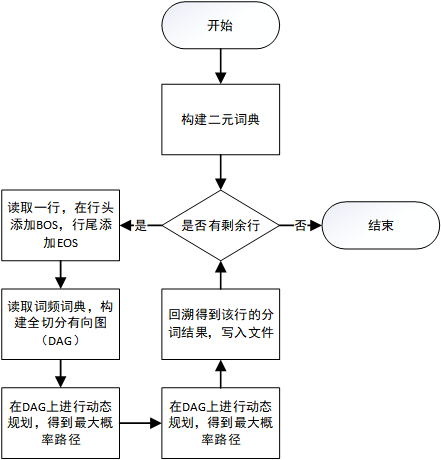
\includegraphics[width=7.5cm]{bigram.png}
		\caption{二元语言模型流程图}\label{bigram_flowpic}
	\end{figure}
	
	\subsection{基于隐马尔科夫模型的分词}
	隐马尔可夫模型(HMM)~\citep{stanke2003gene}是将分词作为字在句子中的序列标注任务来实现的。其基本思路是:每个字在构造一个特定词语时都占据着一个特定的位置即词位,一般采用四结构词位:B(词首),M(词中),E(词尾)和S(单独成词)。比如:
	\begin{quote}
		\verb|“中文/分词/是/文本处理/不可或缺/的/一步/!”|\\
	\end{quote}
	的标注后的形式为
	\begin{quote}
		\verb|“中/B 文/E 分/B 词/E 是/S |\\
		\verb|文/B 本/M 处/M 理/E 不/B |\\
		\verb|可/M 或/M 缺/E 的/S 一/B |\\
		\verb|步/E !/S”|\\
	\end{quote}
	其中,词位序列代表着HMM中不可见的隐藏状态序列,而训练集中的文本则为可见的观测序列。这样就变成了已知观测序列求未知的隐藏序列的HMM问题。
	
	HMM的实现主要分为三步:
	
	\begin{enumerate}
		\item 使用已经分好词的训练集训练HMM模型,计算频数得到HMM的三要素(初始状态概率,状态转移概率和发射概率)。
		\item 使用Viterbi算法以及训练好的三个概率矩阵,将待分词的句子转换为'BMES'类型的状态序列。
		\item 根据已经求出的状态序列,划分句子进行分词。
	\end{enumerate}
	
	\subsection{未登录词的处理}
	分词结果中可能包含了较多单字的分词,而其中大部分都是本应该组成一个词的。出现这个现象的原因是,我们在构建词典时使用的是训练集数据,这使得在对训练集分词时文本中包含了一些没有出现在词典中的未登录词。因此,我们利用隐马尔可夫模型对未登录词进行处理。
	
	\subsection{特殊词的处理}
	对分词结果进行未登录词识别处理之后,虽然各项指标都有了一定程度的提升,但是在文本中仍然存在一些特殊词,如全角英文组成的英文单词、全角数字组成的数词、汉字数字组成的数词等等仍然是以单字的形式存在。本环节的任务就是将这些特殊词进行正确的组合。
	
	特殊词处理程序获取分词结果中连续的单个字,判断其若全为英文字母或全为数字,则将其合并成一个英文单词或一个完整的数词。另外,数字之间可能夹杂诸如“点”、“分之”等字眼,一串数字的末尾可能出现“年”、“月”、“日”、“百”、“千”、“万”等单位,这些字眼也都被纳入考虑的范围,与零散的数字共同组合成一个数词。
	
	
	
	
	
	
	
	
	\section{实验结果}
	\subsection{最大匹配分词实验结果及分析——王雨桐}\label{wyt_analyzation}
	\noindent
	本节将对实现的分词程序的执行效果进行分析。由于使用优化前的分词程序进行分词十分耗时,不能在可接受的时间范围内得出想要的分词结果,因此在本节中讨论分词效果时使用的是第\ref{chapter3.4}节中优化后程序的分词结果。\footnote{\ref{chapter3.2}、\ref{chapter3.4}节中的程序只在词典的查找方法方面有差异,在分词结果上是完全相同的,因此在本节中使用\ref{chapter3.4}节得到的分词结果并不影响分析的严谨性。}
	
	在讨论分词算法的效果时,如果使用整个语料库生成词典,然后再基于该词典对同一篇文本进行分词是很不严谨的,因为词典中的信息和待分词文本的信息重合了,这会造成词典的数据污染,由此得出的分词准确率等指标自然是偏高的,不具有代表性。因此,通常做法是将整篇文本划分为90\%的\textbf{训练集}和10\%的\textbf{测试集}。
	
	\paragraph{训练集、测试集划分规则:}在已经进行过分词和词性标注的语料库文本199801\_seg\&pos.txt中取行数不能被10整除的行作为用于生成词典的\textbf{训练集},在未经分词处理的文本199801\_sent.txt中取行数能被10整除的行作为用于测试分词效果的\textbf{测试集},并在199801\_seg\&pos.txt中取相同位置的行作为分词的标准答案。
	
	\paragraph{判断分词是否正确的代码实现:}由于分词结果与标准答案在文本内容上是一致的,唯一的区别是分词单位的长度有所不同。因此,只需将每个分词的长度做比对,就可以判断分词结果是否正确。伪代码见算法\ref{analysing}。
	
	\begin{algorithm}[ht]
		\caption{统计每行分词结果的正确个数}\label{analysing}
		\begin{algorithmic}[1] %每行显示行号  
			\Require $s$标准分词结果,$m$我的分词结果
			\Ensure $c$正确分词的个数
			\Function{GetNum}{$s, m$}
			\State c $\gets$ 0, i $\gets$0, j $\gets$ 0
			\While{i < \Call{len}{s} and j < \Call{len}{m}}
			\State sl $\gets$ \Call{len}{s[i]}, ml $\gets$ \Call{len}{m[j]}
			\If{sl == ml}
			\State c $\gets$ c + 1
			\Else
			\While{cl != ml}
			\If{sl > ml}
			\State j $\gets$ j + 1, ml $\gets$ \Call{len}{m[j]}
			\Else
			\State i $\gets$ i + 1, sl $\gets$ \Call{len}{s[i]}
			\EndIf
			\EndWhile
			\EndIf
			\State i $\gets$ i + 1, j $\gets$ j + 1
			\EndWhile
			\EndFunction  
		\end{algorithmic}  
	\end{algorithm}
	
	\paragraph{各评价指标的计算方法:}
	\begin{equation}
		\mbox{准确率}=\frac{\mbox{正确分词数}}{\mbox{分词总数}}\label{precision}
	\end{equation}
	\begin{equation}
		\mbox{召回率}=\frac{\mbox{正确分词数}}{\mbox{标准分词数}}\label{recall}
	\end{equation}
	\begin{equation}
		\mbox{F值}=\frac{(k^2+1)\times \mbox{准确率}\times \mbox{召回率}}{k^2\times \mbox{准确率}+\mbox{召回率}}\label{fvalue}
	\end{equation}
	
	使用以上统计算法以及计算公式,计算出在测试集中FMM和BMM算法分词结果的准确率、召回率和F值(k取1)分别如下:
	\begin{table}[htb]
		\centering
		\begin{tabular}{lrrr}
			\hline \textbf{算法} & \textbf{准确率} & \textbf{召回率} & \textbf{F值}\\ \hline
			HMM & 88.1518\% & 93.0735\% & 90.5458\%\\
			BMM & 88.3553\% & 93.3600\% & 90.7887\%\\
			\hline
		\end{tabular}
		\caption{\label{p_r_f_table} 分词结果指标对比 }
	\end{table}
	通过表\ref{p_r_f_table}可以发现,不论是准确率还是召回率,BMM算法获得的结果都要略优于HMM算法。我认为造成这一结果的主要原因有以下几方面:
	\paragraph{汉语中的偏正结构}
	在汉语中,偏正结构是一类十分常见的结构。在构成一个名词时,使用定语+中心词的偏正结构构成一个偏正短语的现象是十分普遍的,如“实验报告”、“产品质量”、“中国企业”等等。这些短语的共同点,都是由前一个词作为定语修饰位于后方的中心词。因此,在给定一个词时,在名词的后方再添加少量的字,组成一个偏正短语是十分容易的,这便容易在对句子进行正向分词解析的过程中造成歧义效果。例如,如果遇到下面的句子:
	\begin{quote}
		\verb|“研究生命的起源”|\\
	\end{quote}
	其中“研究”已经构成了一个词,然而,当我们在其后面由填上一个“生”字之后,又可以构成偏正短语“研究生”,如果将“研究生”作为一个分词,也是说得通的。如果我们采用FMM分词算法,则在两个歧义的选择中更偏向于长度更长的后者,分词结果也变成了“研究生/ 命/ 的/ 起源”。换句话讲,大量存在于汉语当中的偏正短语有时会混淆FMM算法的判断,让其容易掉进歧义的陷阱。相反,如果我们使用BMM算法,后方的词会优先抢占原先可以组成偏正结构的一些字,排除了可能的歧义。再者,在已知的词之前填上少量的词,能够组成新的短语的难度要明显大于在后方填入,因此BMM中产生的歧义也会少于FMM。于是使用BMM更易得到正确的分词结果,即“研究/ 生命/ 的/ 起源”。
	\begin{table*}[h]
		\centering
		\begin{tabular}{l|llllll}
			\hline
			\textbf{词频(次)}  & 400  & 200  & 50   & 20    & 2     & 1      \\ \hline
			\textbf{占比(\%)} & 0.91 & 1.74 & 5.63 & 10.93 & 55.04 & 100.00 \\ \hline
		\end{tabular}
		\caption{词典中词频大于等于一定值的词数占比}
		\label{sxy:t1}
	\end{table*}
	\begin{table*}[h]
		\centering
		\begin{tabular}{cccccc}
			\hline
			\textbf{Algorithm}            & \textbf{Precision (\%)} & \textbf{Recall (\%)}   & \textbf{F}             & \textbf{Optimization} & \textbf{Time (s)} \\ \hline
			\multirow{4}{*}{FMM} & \multirow{4}{*}{93.98}  & \multirow{4}{*}{94.5}  & \multirow{4}{*}{94.24} & -                     & 22195.06          \\
			&                         &                        &                        & Trie+AVL              & 15.01             \\
			&                         &                        &                        & Trie+HASH1            & 300.63            \\
			&                         &                        &                        & Trie+HASH2            & 9.12              \\ \hline
			\multirow{4}{*}{BMM}          & \multirow{4}{*}{94.23}  & \multirow{4}{*}{94.72} & \multirow{4}{*}{94.47} & -                     & 22179.69          \\
			&                         &                        &                        & Trie+AVL              & 13.63             \\
			&                         &                        &                        & Trie+HASH1            & 221.57            \\
			&                         &                        &                        & Trie+HASH2            & 8.27              \\ \hline
		\end{tabular}
		\caption{正反向最大匹配分词结果}
		\label{sxy:t2}
	\end{table*}

	\paragraph{汉语中的主谓结构}
	汉语中另一类常见的结构是主谓结构,这一结构大量出现在各种句子中。而谓词有一种十分明显的趋向,即多数是由复数个字构成的,如“学习”、“工作”、“欢呼”等等。此时如果使用BMM算法,会将尽可能多的字分配给主谓结构中的谓语,这满足了谓语动词通常由多个字组成的特点。相反,如果使用FMM算法,算法倾向于分配给主语更多的字,这样很可能造成没有足够多的字构成谓语。结合上面的理论,分配给主语更多的字,反而更容易引起歧义,造成准确率的下降。这里给出一个具体的例子:
	\begin{quote}
		\verb|“鞭炮声响彻夜空”|\\
	\end{quote}
	在这个句子中,“鞭炮声”是主语,“响彻”是谓语且由两个字构成。使用FMM,很容易将其分解成“鞭炮声响/ 彻/ 夜空/”,这里将“响”字分配给主语后,留给谓语的只剩一个字了,这与我们的语言习惯是相悖的,因为汉语中很少使用单个字组成的谓语动词。而使用BMM算法,则可优先将“响”分配给谓语构成“响彻”,这样便可以得到正确的分词结果“鞭炮声/ 响彻/ 夜空/ ”。
	
	
	
	\subsection{最大匹配分词实验结果——石翔宇}
	使用\ref{sxy:mec}节中的统计算法以及计算公式,我们将各个算法的分词结果进行比较与分析。
	
	\subsubsection{词典构建结果}
	
	
	
	对词典的词频统计如表\ref{sxy:t1}所示。我们可以看到词频大于等于400次的词仅占了0.91\%,词频大于等于20次的词也只有10.93\%。而词频大于等于2次的词占到了55.04\%,绝大多数的词仅出现了一次。我们可以看到出现次数和词频的对数大致呈负对数的关系,二者之间可能可以用一个函数关系来拟合。
	
	\subsubsection{正反向最大匹配分词结果}
	
	
	
	正反向最大匹配分词结果如表\ref{sxy:t2}所示。我们可以看到,不论是准确率、召回率还是F值,BMM算法获得的结果都要优于HMM算法。
	
	与此同时,改进的词典结构也极大地提升了算法的速度。从优化前算法需要上万秒到优化后十秒内就能跑完,可以看出合适的数据结构对算法的重要性。
	
	\subsection{最大匹配分词实验结果——林燕燕}
	
	\subsubsection{正反向最大匹配分词——最少代码结果}
	由于使用最少代码量代码,并未对数据结构及查找算法进行优化,对十分之一的测试集需要半个小时才能运行结束,则对于所有文本则需四到五个小时,效率非常低。
	
	
	\subsubsection{正反向最大匹配分词效果分析结果}
	\begin{table}[htb]
		\centering
		\begin{tabular}{ccc}
			\hline
			& \textbf{FMM} & \textbf{BMM} \\ \hline
			\textbf{正确分词数}    & 1085485      & 1088184      \\
			\textbf{标准分词数}    & 1140931      & 1140931      \\
			\textbf{模型分词数}    & 1174256      & 1175022      \\
			\textbf{准确率 (\%)} & 92.44        & 92.61        \\
			\textbf{召回率 (\%)} & 95.14        & 95.38        \\
			\textbf{F值}       & 93.77        & 93.97        \\ \hline
		\end{tabular}
		\caption{正反向最大匹配分词结果}
		\label{lyy:t1}
	\end{table}
	\begin{table*}[htb]
		\centering
		\begin{tabular}{cccc}
			\hline
			算法  & 优化前用时 (s) & 优化后用时 (s) & 优化比例 (\%) \\ \hline
			FMM & 1898.02   & 14.02     & 99.26     \\
			BMM & 1775.86   & 9.02      & 99.49     \\ \hline
		\end{tabular}
		\caption{速度优化结果}
		\label{lyy:t2}
	\end{table*}
	\begin{table*}[!htb]
		\centering
		\begin{tabular}{ccccc}
			\hline
			& \textbf{额外处理} & \textbf{准确率} & \textbf{召回率} & \textbf{F值} \\ \hline
			\multirow{3}{*}{一元文法} & -             & 94.35        & 96.22        & 95.28       \\
			& 处理未登录词        & 94.95        & 96.23        & 95.58       \\
			& 处理未登录词和特殊词    & 94.98        & 96.21        & 95.59       \\ \hline
			\multirow{3}{*}{二元文法} & -             & 70.41        & 94.54        & 80.71       \\
			& 处理未登录词        & 70.8         & 94.48        & 80.94       \\
			& 处理未登录词和特殊词    & 93.77        & 96.1         & 94.92       \\ \hline
		\end{tabular}
		\caption{统计语言模型分词结果}
		\label{t}
	\end{table*}
	
	正反向最大匹配分词结果如表\ref{lyy:t1}所示。FMM和BMM的分词效果存在一定性能差异,且均是BMM效果较好。
	
	这是由于汉语中偏正结构较多,从后向前匹配,可以适当提高精确度。所以,反向最大匹配法比正向最大匹配法的误差要小。统计结果表明 ,使用正向最大匹配的错误率为 1/169,使用反向最大匹配的错误率为 1/245。例如切分字段“硕士研究生产”,正向最大匹配法的结果会是“硕士研究生 / 产”,而逆向最大匹配法利用逆向扫描,可得到正确的分词结果“硕士 / 研究 / 生产”。
	
	\subsubsection{基于机械分词系统的速度优化结果}
	
	对代码中数据结构和查找算法进行了优化,使用字典树加哈希值进行优化,得到结果如表\ref{lyy:t2}所示。
	
	可以看到时间得到了极大的优化,且BMM消耗时间更少。
	
	\subsection{统计语言模型实验结果}
	统计语言模型实验结果均使用k-折交叉验证获得。
	\subsubsection{n元文法的实验结果}
	表\ref{t}中展示了一元文法和二元文法的分词结果。可以看出,朴素的二元文法的效果远远不及一元文法的效果,这可能是二元文法词典的稀疏性所导致的。朴素的一元文法的分词结果有着较高的水准。
	
	\subsubsection{未登录词的处理}
	
	表\ref{t}中展示了进行未登录词处理后的分词结果。可以看出,将一元语言模型和二元语言模型的分词结果进行未登录词处理后,各项指标均有了一定的提升,但提升不大。
	
	\subsubsection{特殊词的处理}
	表\ref{t}中展示了进行特殊词处理后的分词结果。一元、二元语言模型在进行了前面的未登录词识别的基础之上,进一步进行特殊词处理后又可获得进一步的性能提升。一元文法的提升不大,因为一元文法的效果已经很好;而二元文法的提升很大。

\bibliographystyle{acl_natbib}
\bibliography{anthology,acl2021}
	
\end{document}